\documentclass[thesis.tex]{subfile}

% Purpose of background chapter
% 1. Background to understand thesis (short)
% 2. "Related work", or intro++: research context, where the boundaries are

% Examiners will know about: PDEs, maybe handcoding

\chapter{Background and related work}
\label{ch:background}

% TODO: \ref sections here
We first provide an overview of loop nest optimisations, techniques, and analyses that we have applied, with specific reference to the polyhedral model. % TODO: cite
This forms the basis and context for the entire report, and in particular informs our overview of Devito (Section~\ref{sec:devito}) and the survey of related work, which composes the remainder of this chapter (Section~\ref{sec:survey}).

% TODO: grandiose
This project extends a well-established idea from compiler theory, \emph{tiling}, to another dimension (time) in Devito.
This has traditionally been a challenging problem, as evaluating data dependences efficiently is beset with difficulties.

% We have a tradeoff between computation and memory usage
% Big IDEA: can use more memory, less computation ("this really should be true")
% Project: optimise memory usage
% Why exciting: one step to proving the idea


\section{Loop tiling}
\label{sec:bg-loop-tiling}
% TODO: mention that iteration spaces under consideration are (nice rectangular continuous) matrices

\subsubsection{Optimisations on loop nests}
The bulk of computation for finite difference methods lies in loops. % TODO: cite
Loop nest optimisations seek to transform a loop, possibly changing its execution order to use data locality, parallelism, or otherwise avoid unnecessary operations.

\subsection{Insight}
To exploit data locality, we must use data before it gets evicted from the cache; ideally, data is not loaded into the cache more than once.
This is a complex process \cite{lam91}; nevertheless reuse does occur within sufficiently small iteration spaces.
We therefore contrive small iteration spaces by partitioning the original space into smaller tiles (Figure~\ref{fig:tiled-space}).

\begin{figure}[ht]
	\centering
	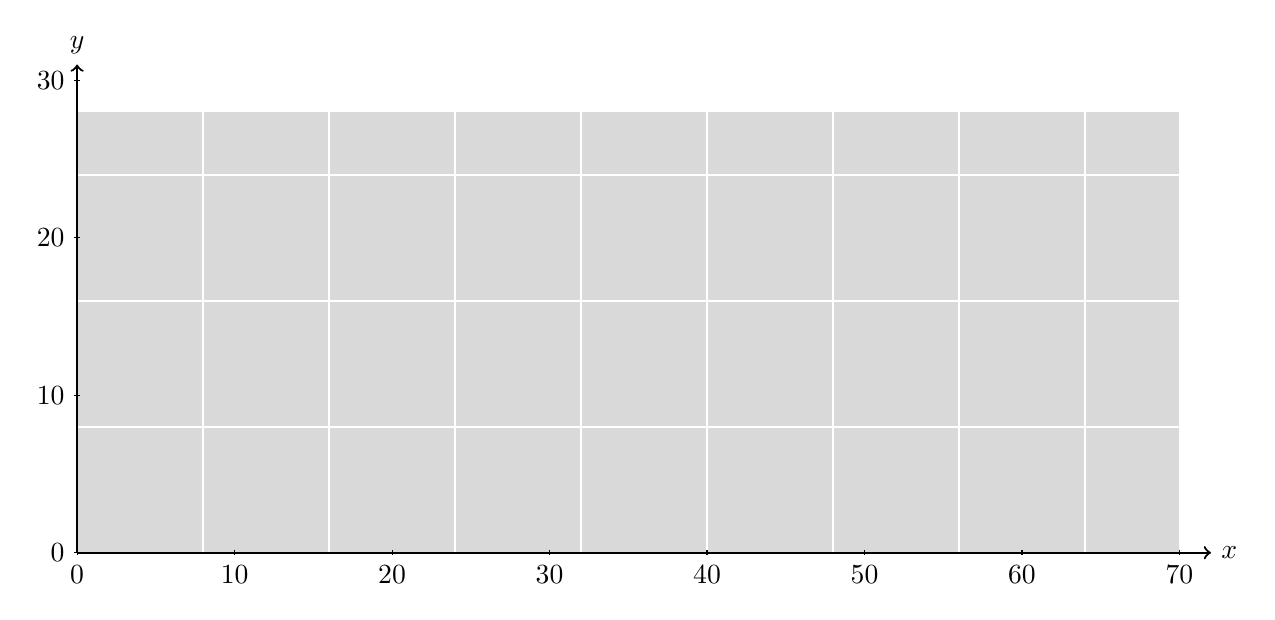
\begin{tikzpicture}
	\fill[gray!30!white] (0,0) rectangle (14,5.6);
	\draw[step=1.6cm,white,thick] (0,0) grid (14,5.6);

	\draw[thick,->] (0,0) -- (14.4,0) node[right]{$x$};
	\draw[thick,->] (0,0) -- (0,6.2) node[above]{$y$};
	\foreach \x in {0,10,20,30,40,50,60,70}
		\draw (\x*0.2 cm,1pt) -- (\x*0.2 cm,-1pt) node[anchor=north] {$\x$};
	\foreach \y in {0,10,20,30}
		\draw (1pt,\y*0.2 cm) -- (-1pt,\y*0.2 cm) node[anchor=east] {$\y$};
	\end{tikzpicture}
	\caption{Tiles over an iteration space. Note that the tile size need not be the same in each dimension, or divide the extent of the iteration cleanly.}
	\label{fig:tiled-space}
\end{figure}

Loop tiling is also commonly known as \emph{blocking}, or perhaps less transparently \emph{strip-mine and interchange}, as tiling is typically achieved through these two transformations.

\paragraph{Additional motivation}
As a remark, the stencils resulting from finite-difference methods tend to have high \emph{arithmetic} intensity, while tiling is used to reduce \emph{memory} pressure.
As we note later, we can decrease arithmetic intensity (at the expense of increasing memory pressure) by eliminating common sub-expressions, which would ordinarily result in redundant computation.
Further, tiling may also enable other transformations, such as loop-invariant code motion, which again reduces redundant computation.

\subsection{Strip-mining}
\begin{figure}[ht]
\begin{lstlisting}
for (int x = x_start + 1; x < x_end - 1; x++) {
  A[x] = B[x-1] + B[x+1];
}

for (int x_blk = x_start + 1; x_blk < x_end - 1; x_blk += x_blk_size) {
  for (int x = x_blk; x < min (x_end - 1, x_blk + x_blk_size); x++) {
    A[x] = B[x-1] + B[x+1]; // loop body unchanged
  }
}
\end{lstlisting}
	\caption{A regular loop, then strip-mined over the variable \texttt{x}. Offsets are used on \texttt{x\_start}, \texttt{x\_end} to prevent out-of-bounds accesses. The \texttt{min} function avoids the need for remainder loops, in case the tile (block) size does not evenly divide the extent of the iteration. We will abbreviate the variable names in further examples.}
	\label{lst:stripmine-basic}
\end{figure}

Named after the mining practice, strip-mining involves dividing a dimension of the iteration space into strips (Figure~\ref{lst:stripmine-basic}).\footnote{However, you cannot divide a dimension into lateral strips, only sequential ones.}
By itself, strip-mining does not change the execution order; it is a gateway to further transformations.

We will need more loops to perform an interchange.
Figure~\ref{lst:stripmine} illustrates a loop that has been strip-mined in two dimensions.

\begin{figure}[ht]
	\begin{lstlisting}
for (int x_blk = x_s; x_blk < x_e; x_blk += x_bs) {
  for (int x = x_blk; x < min(x_e, x_blk + x_bs); x++) {
    for (int y_blk = y_s; y_blk < y_e; y_blk += y_bs) {
      for (int y = y_blk; y < min(y_e, y_blk + y_bs); y++) {
        A[x][y] = B[x][y] + B[x][y+1];
      }
    }
  }
}
	\end{lstlisting}
	\caption{Strip-mining a loop nest iterating over variables \texttt{x} and \texttt{y}. Offsets have been omitted here.}
	\label{lst:stripmine}
\end{figure}

% TODO: consider visualising the iteration space here

\subsection{Loop interchange}
\label{sec:interchange}
Loop interchange is based on the observation that a change in execution order does not change the correctness of a strip-mined program.
We will change the order of the loops to iterate over the tiles, then within them (Figure~\ref{lst:interchange}).

\begin{figure}[ht]
\begin{lstlisting}
for (int x_blk = x_s; x_blk < x_e; x_blk += x_bs) {
  for (int y_blk = y_s; y_blk < y_e; y_blk += y_bs) {
    for (int x = x_blk; x < min(x_e, x_blk + x_bs); x++) {
      for (int y = y_blk; y < min(y_e, y_blk + y_bs); y++) {
        A[x][y] = B[x][y] + B[x][y+1];
      }
    }
  }
}
\end{lstlisting}
	\caption{The loop nest of Figure~\ref{lst:stripmine}, with the \texttt{x} and \texttt{y\_blk} loops interchanged.}
	\label{lst:interchange}
\end{figure}

This is valid when each point in the iteration space does not depend on the values calculated in the same iteration.
Therefore, one must be extremely careful that no data dependences cross boundaries between tiles; if they do, they must be permitted to cross only in one direction, and the tiles must be scheduled in that order.


\section{Tiling in the time dimension}
\label{sec:bg-time-tiling}

\subsection{Motivation}
% TODO: vague; so what?
Many problems involving finite difference methods are computationally bounded, rather than bounded by memory throughput.
However, it is possible to reduce the operation count by exploiting the structure of expressions computed at the cost of increased memory pressure~\cite{fabio-memory}.
We are therefore interested to perform time-tiling to realise significant performance gains, possibly 27.5\% in Devito alone~\cite{dylan}.
This improvement is significant over the optimisation from tiling in all dimensions apart from time~\cite{pluto}.

\subsection{Skewing}
In Section~\ref{sec:interchange} we stated that interchange is valid when data dependences do not cross boundaries between tiles.
This is clear, as if there are no inter-tile dependences, the tiles can be executed in any order.

% TODO: "problems we discuss later": verify these are indeed discussed
% This could probably be clearer
\emph{Data dependences} occur when two statements reference a datum, at least one of which change it.
To preserve the dependence, we must preserve the order in which these statements are executed.
Figure~\ref{fig:dependence} illustrates how dependences may look in a (1-dimensional) iteration space similar to the problems we discuss later.

\begin{figure}[ht]
	\centering
	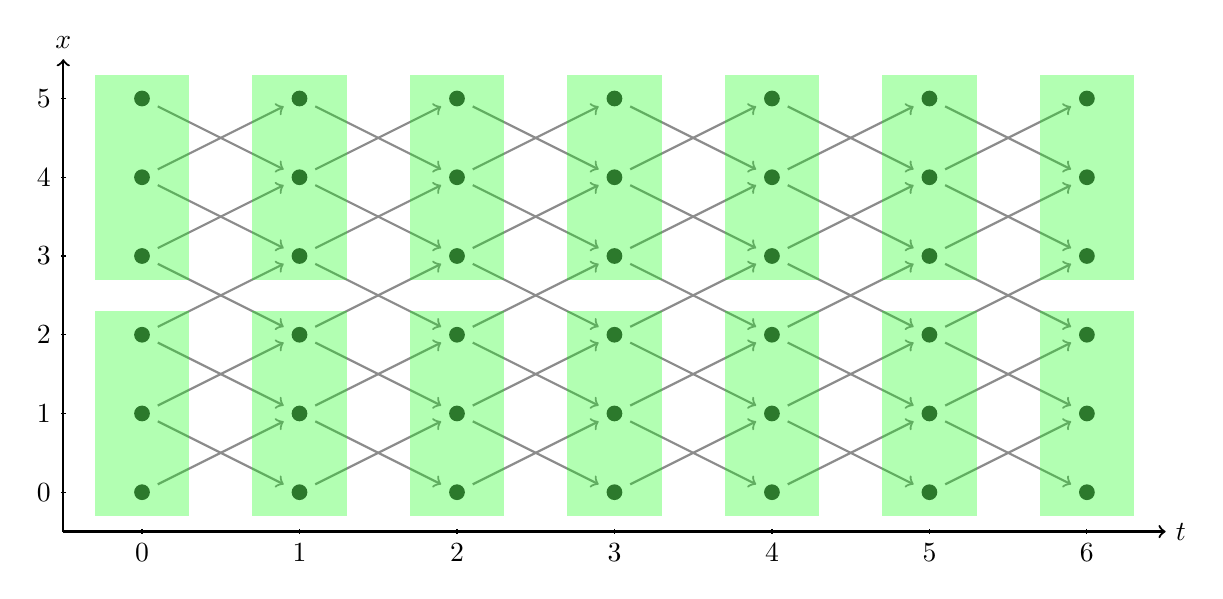
\begin{tikzpicture}
	\draw[thick,->] (-1,-.5) -- (13,-.5) node[right]{$t$};
	\draw[thick,->] (-1,-.5) -- (-1,5.5) node[above]{$x$};

	\foreach \t in {0,1,2,3,4,5,6}
	\foreach \x in {0,1,2,3,4,5}
		\fill[darkgray] (\t*2,\x) circle (0.1);

	\foreach \t in {0,1,2,3,4,5}
	\foreach \x in {1,2,3,4,5}
		\draw[thick,->,darkgray!60] (\t*2+.2,\x-.1) -- (\t*2+1.8,\x-.9);

	\foreach \t in {0,1,2,3,4,5}
	\foreach \x in {0,1,2,3,4}
		\draw[thick,->,darkgray!60] (\t*2+.2,\x+.1) -- (\t*2+1.8,\x+.9);

	\foreach \t in {0,1,2,3,4,5,6}
	\foreach \x in {0,3}
		\fill[green,opacity=0.3] (\t*2-.6,\x-.3) rectangle (\t*2+.6,\x+2.3);

	\foreach \t in {0,1,2,3,4,5,6}
		\draw (\t*2,1pt-.5cm) -- (\t*2,-1pt-.5cm) node[anchor=north] {$\t$};
	\foreach \x in {0,1,2,3,4,5}
		\draw (1pt-1cm,\x) -- (-1pt-1cm,\x) node[anchor=east] {$\x$};
	\end{tikzpicture}
	\caption{An iteration space with data dependences indicated by a forward arrow for a value derived from a dependence. It would not be valid to interchange loops over the \texttt{t} and \texttt{x} dimensions here.}
	\label{fig:dependence}
\end{figure}

We employ skewing to make the interchange valid (Figure~\ref{fig:dependence-skew}).
This solves the dependency problem~\cite{boulet98}.

% TODO: vague
\begin{figure}[!ht]
	\centering
	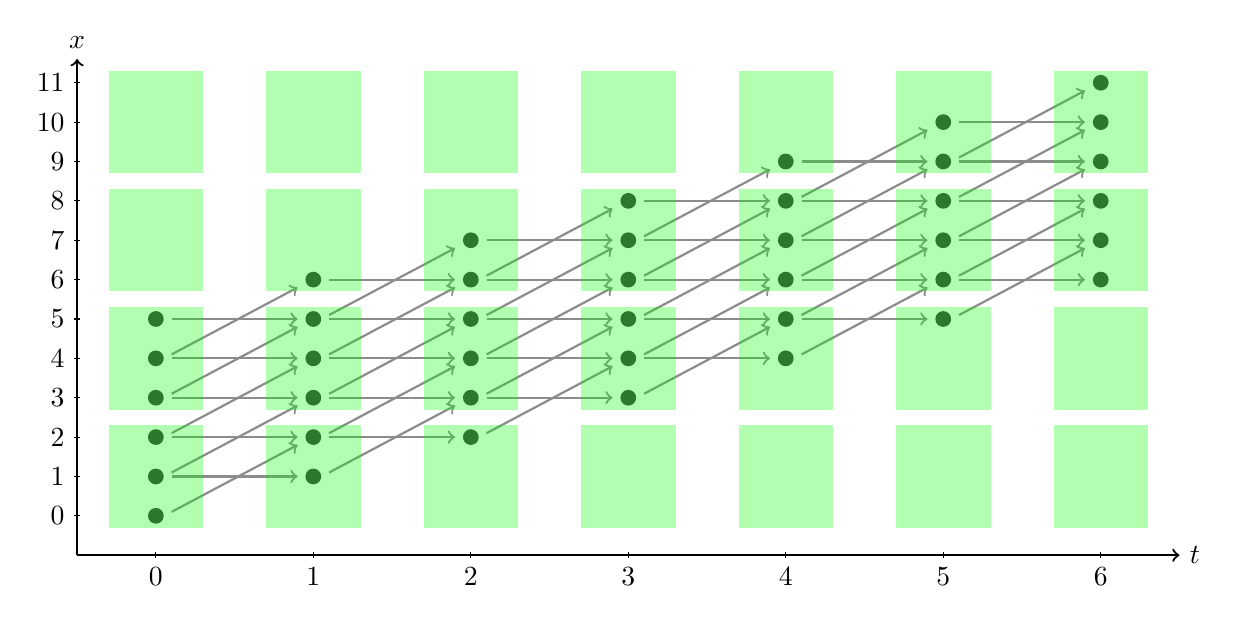
\begin{tikzpicture}
	\draw[thick,->] (-1,-.5) -- (13,-.5) node[right]{$t$};
	\draw[thick,->] (-1,-.5) -- (-1,5.8) node[above]{$x$};

	\foreach \t in {0,1,2,3,4,5,6}
	\foreach \x in {0,1,2,3,4,5}
		\fill[darkgray] (\t*2,\x/2+\t/2) circle (0.1);

	\foreach \t in {0,1,2,3,4,5}
	\foreach \x in {1,2,3,4,5}
		\draw[thick,->,darkgray!60] (\t*2+.2,\x/2+\t/2) -- (\t*2+1.8,\x/2+\t/2);

	\foreach \t in {0,1,2,3,4,5}
	\foreach \x in {0,1,2,3,4}
		\draw[thick,->,darkgray!60] (\t*2+.2,\x/2+\t/2+.05) -- (\t*2+1.8,\x/2+\t/2+.9);

	\foreach \t in {0,1,2,3,4,5,6}
	\foreach \x in {0,3,6,9}
		\fill[green,opacity=0.3] (\t*2-.6,\x/2-.15) rectangle (\t*2+.6,\x/2+1.15);

	\foreach \t in {0,1,2,3,4,5,6}
		\draw (\t*2,1pt-.5cm) -- (\t*2,-1pt-.5cm) node[anchor=north] {$\t$};
	\foreach \x in {0,1,2,3,4,5,6,7,8,9,10,11}
		\draw (1pt-1cm,\x/2) -- (-1pt-1cm,\x/2) node[anchor=east] {$\x$};
	\end{tikzpicture}
	\caption{The same iteration space skewed by a factor of \texttt{t} in the \texttt{x} dimension. Note that the tiling is now valid and we can execute the tiles in either dimension first, and that we can merge tiles in the \texttt{t} dimension.}
	\label{fig:dependence-skew}
\end{figure}


\section{Devito}
\label{sec:devito}

Devito~\cite{devito} is a domain-specific language and code generation framework for finite-difference method computations~\cite{devito-web}.
Its main use case is building solvers for differential equations from high-level mathematical expressions, written using the symbolic library \emph{SymPy}, and is targeted at the domain of seismic imaging.


\subsection{Motivation}
Efficient computation demands that we are able to use every optimisation at our disposal.
As architecture for computation changes, introducing new instructions, GPUs and distributed systems, specialist research compilers using just a handful of related optimisations do not suffice for high-performance applications.

An equal part of optimisation is reducing the turnaround time in modelling.
Providing an interface that domain specialists are familiar with reduces friction, and removes the need to construct stencils by hand.
This also reduces errors by simplifying the inputs that they provide.

This combination of ease of use through the Python and \emph{SymPy} interface and the generation of optimised and fast C code without user intervention make Devito an attractive tool.


\subsection{Domain-specificity}
Polyhedral compilers such as PLUTO~\cite{pluto}, with its backend CLooG~\cite{cloog-isl} are able to apply tiling over generic loop nests.
Further, the iteration spaces which they handle are unions of convex polyhedra, again far more general than the use cases Devito is likely to encounter.
This generality is not necessary when merely applying finite-difference methods to solve differential equations, not least when targeting a specific domain which uses such methods.

We can instead make use of this specificity to make informed choices in our optimisations, or streamline an auto-tuning routine.
Further, we are able to combine different optimisations, at the stencil level and progressively lower levels.
Finally, considering likely use cases, it may be desirable to target compilation for architectures not supported by more general compilers, such as GPUs.


\subsection{Layers of abstraction}
The separation of symbolic expressions and the underlying C code to which they are compiled is key to Devito's comprehensibility and usage.
By progressive manipulation, optimisation and modification is possible at many layers.
A further benefit as a more general software engineering practice is the possibility of small unit tests for individual components.

This also allows the integration of other tools, which may fit a user's needs better, and enables easy benchmarking of Devito's performance against said tools.
For instance, YASK (Section~\ref{sec:yask}) is being integrated as a compilation backend.

An important feature for seismic imaging is sparse-point interpolation.
Devito handles this by exposing powerful lower-level APIs to allow the construction of comprehensive representations which would be tedious or impossible at higher levels of abstraction.


\subsection{Architecture}
The Devito compilation process (Chapter~\ref{ch:devito}) can be divided into several stages:

\begin{enumerate}
	\item Construction of stencil equations (symbolic kernel)
	\item Grouping of expressions
	\item CSE and indexing of stencil (the Devito symbolic engine, Section~\ref{sec:dse})
	\item Loop optimisation and other transformations (the Devito loop engine, Section~\ref{sec:dle})
	\item Code generation
\end{enumerate}

Our time-tiling transformation will occur in the DSE and DLE, covered in detail in the respective sections.


\section{Survey of related work}
\label{sec:survey}

The following sections provide an overview of tools related to Devito and of interest to our investigation.
In particular, they identify instances of time-tiling (or equivalent transformations) which have been solved and the insights required, and analyse their applicability to time-tiling in Devito.


\subsection{Halide}
Halide was conceived as a representation for image processing pipelines.
Many image processing algorithms are similar to stencils: Halide specifically deals with overlapping stencils; this overlap can be compared to iteration in the time dimension.

\subsubsection{Insight}
It is possible to separate image processing algorithms (``filters'') and their schedules~\cite{halide12}.
Optimisation for an architecture then becomes an exercise in optimising the schedule and not the filters, which are reduced to kernels.\footnote{See {https://github.com/halide/CVPR2015/blob/master/blur.cpp} for an example}
Halide is therefore a stencil compiler.

Modifying schedules is analogous to our loop optimisations: filters can be vectorised, tiled, interchanges are possible, etc.
Halide further provides an auto-tuner which estimates, among other things, arithmetic intensity of filters and loop transformations which Devito also employs~\cite{halide13,halide-sched}.
Part of its analysis examines the trade-off between additional computation and memory traffic.

\subsubsection{Applicability}
The problem domain, image processing, that Halide is concerned with may appear very different to that of differential equations.
However, the underlying natures of the solutions are very similar: use of stencil kernels, trade-off between redundant computation and memory pressure, etc.
Analogously to time-tiling, Halide is able to compute tiles across filters.

Likewise, in Devito, \emph{each time iteration} may contain several stencil kernels applied consecutively.
To extend the analogy, Halide is concerned with tiling within \emph{a single} timestep, while this project investigates tiling over \emph{multiple} timesteps.

Domain-specific frameworks bring insight to a problem which general-purpose compilers may not possess; the separation of algorithm and schedule, while touted as novel, is essentially what every compiler applies during transformations such as loop interchange.


\subsection{Pochoir}
Pochoir is a compiler for stencil computations focussed on utilising parallelism and multithreading.
Stencils are defined with provided C++ templates, from which the computations are generated.
Pochoir implements a two-phase compilation strategy: the first involves compilation with the Pochoir template library, which ensures compliance and compatibility with the library. At this stage, one may debug the non-optimised code.
The second is the optimisation phase using the Pochoir compiler\footnote{The Pochoir compiler will also invoke the user's Cilk Plus compiler.}~\cite{pochoir}.

\subsubsection{Insight}
\paragraph{Cache-oblivious algorithms}
These seek to eliminate tuning of cuts (tile size) based on cache properties including cache sizes or replacement policies, reasoning that the correct cache-oblivious algorithm will achieve (asymptotically) the same performance~\cite{frigo-cacheoblivious}.

Pochoir uses a cache-oblivious algorithm based on parallel cuts.
These \emph{hyperspace} and \emph{time cuts} decompose the iteration spaces (``zoids'') into smaller spaces recursively;
they are chosen to improve parallelism while maintaining cache efficiency~\cite{frigo-cacheoblivious-alg}.

Thanks to cut dependence analysis, the resultant trapezoids can span iterations of a time loop. Note that the domain which Pochoir operates on are unions of convex polyhedra, which are more general than the hypercube-like iteration spaces described so far.

\subsubsection{Applicability}
The Cilk Plus framework, which Pochoir uses, is intended to produce optimal scheduling for parallel tasks, and cache-oblivious algorithms may be optimal up to a constant factor, which would be interesting when targeting multiple platforms.
Nevertheless, significant speedup can occur with \emph{cache-aware} algorithms, which employ tuning for multiple levels of cache~\cite{kowarschik-cacheaware}.
Indeed, due to a difficulty in choosing suitable base case sizes for the interior trapezoids, Pochoir includes an auto-tuner for this purpose.
This is especially significant to domain specialists who are experimenting and changing models, or those who are performing stencil computations over large iteration spaces.

Finally, the Cilk Plus framework is in the process of deprecation~\cite{cilkplus-migrate-web}, and Pochoir is not presently maintained.
While the concepts behind it may be sound and applicable in specific circumstances, it would be unsuitable for integration with Devito.


\subsection{YASK}
\label{sec:yask}

\emph{Yet Another Stencil Kernel} is a framework from Intel Corp. that transforms and optimises stencil kernels, especially targeting the Xeon Phi platform~\cite{yask-web}.
Like Pochoir, YASK provides C++ templates for stencils.
Similarly to Halide, it uses a genetic-algorithm based search for its auto-tuner.

It is intended to function both as a platform for domain specialists to experiment with (higher-level) optimisations, as well as for the compilation of high-performance kernels.

\subsubsection{Insight}
Stencil kernels rapidly grow complicated.
Once optimisations have been applied (possibly through a specialised stencil compiler) to stencils, general-purpose compilers are less able to explore the trade-offs of further optimisation which they would ordinarily apply, such as parallelism.
YASK aims to solve this by, among other things, implementing a two-stage compiler (stencils and loops) and tuning for the execution environment~\cite{yask-paper}.
We draw a comparison to Devito here.

In contrast to polyhedral research compilers such as PLUTO~\cite{pluto}, YASK has a specific focus on combining optimisations such as vector folding~\cite{yount-vector} with the loop optimisations which they perform.

\subsubsection{Applicability}
YASK was originally created to implement vector folding, a technique which simultaneously takes advantage of SIMD instructions and reduces memory bandwidth usage.
This is especially relevant in Devito, which has the transformation of arithmetically intensive computations into memory intensive computations as a basis.

Further, with its emphasis on integrating different optimisations, rather than investigating them separately, YASK is a practical tool for a workflow involving stencils.
There would be no need to apply a separate stencil compiler, then a polyhedral compiler, without the guarantee that the latter would understand and be able to build open the complexities introduced by the former.
One might remark, however, that the same applies when constructing stencils from differential equations: instead they are reduced to a form (C++ templates) that the compiler understands.

As noted in Section~\ref{sec:devito}, Devito is in the process of integrating YASK as a compilation backend.


\subsection{Firedrake}
Firedrake is a tool for solving partial differential equations on unstructured meshes using the \emph{finite-element method}~\cite{firedrake}.
It is aimed at simulation and modelling of systems through PDEs, notably separating optimisations into different layers of abstraction.

FEniCS~\cite{fenics}, another tool in the domain of finite-element solvers, separates the usage of finite-element methods and their implementation; Firedrake takes this a step further while retaining the domain-specific language and focus which it derives.

\subsubsection{Insight}
Successfully optimising the solution of PDEs involves expertise at many levels, from numerical analysis of the equations and mesh generation, to the loop optimisations discussed here.
Just as we separate stencil optimisations from polyhedral ones, we should also abstract these layers.

Again, this makes the \emph{optimised} solution of partial differential equations accessible to domain specialists without particular expertise in computer architecture, transformation of expressions into efficient kernels~\cite{coffee}, or mesh generation.

\subsubsection{Applicability}
Through its many layers of abstraction, Firedrake provides a natural way to access lower-level structures such as kernels and the underlying data structures.
Like Devito, this allows specialists to manipulate the computation not just at the highest level of the model, but also at levels which the specialist may have insight to, but would not be otherwise exposed.

While many of the problems which Firedrake deals with are not directly related to Devito (such as unstructured meshes), the concept of abstraction is sound and very relevant to software engineering.
Of particular relevance is the granularity to which abstractions are helpful at the lower levels in which we are interested, the use of kernels (albeit not stencils), and the discretisation of operators.

Hence Firedrake comes far closer to Devito than the previously-discussed tools, as it covers the full process of computation, from the models and differential equations rather than the resultant kernels.
Although the main optimisation that we discuss, time tiling, functions at the kernel level, Firedrake gives a broader view of the context of the problem to be solved, and the model in which Devito resides.


\section{Summary}
In this chapter, we have given an overview of the core optimisation concepts explored and terminology used throughout this work.
Further, we discussed the motivation and context of Devito specifically, its overall architecture and usage, and the importance of the time-tiling transformation; these will inform our evaluation (Chapter~\ref{ch:evaluation}).
Finally, we have examined related work in the form of tools employing transformations relevant to time-tiling and stencil computations, and most importantly, the insights which they bring to our implementation (Chapter~\ref{ch:implementation}).
